After installing the \mitobo jar archive with all its dependencies \mitobo adds a new entry 
denoted 'MiToBo' to ImageJ's plugin menu from where you have access to \mitobo's functionality 
(Fig.~\ref{fig:imageJ}). It basically subsumes an option 'MiToBo Runner' to open \mitobo's 
operator runner which grants access to all \mitobo operators (see below), and an item 
'Grappa Editor' to invoke the graphical workflow editor (Sec.~\ref{sec:grappa}). In
addition, there might appear some more items. All of them are related to so-called 'quick start
plugins'. These ImageJ plugins allow direct access to some interesting operators (and some few
real plugins) in \mitobo 
dedicated to specific applications or techniques. Among those are for example
\begin{itemize}
  \item the {\tt 'Scratch Assay Analyzer'} which is a tool for quantifying gap development in 
  	scratch assay images as used in cell migration experiments \cite{Glass12_PR, Glass12_ImageJ},
  \item the {\tt 'Snake Optimizer'} which features an implementation of parametric active contours
  	and in particular allows for interactive evaluation of various energy models
  	\cite{Moeller12_IJ},
  \item {\tt 'Threshold Image'} which is an interactive image thresholder,
  \item and finally the two plugins {\tt 'Open Image MTB'} and {\tt 'Save Image MTB'} which allow
  	for image I/O considering extracted processing histories (cf.~Chap.~\ref{sec:history}).  
\end{itemize} 
\begin{center}
\begin{figure}[t]
\begin{center}
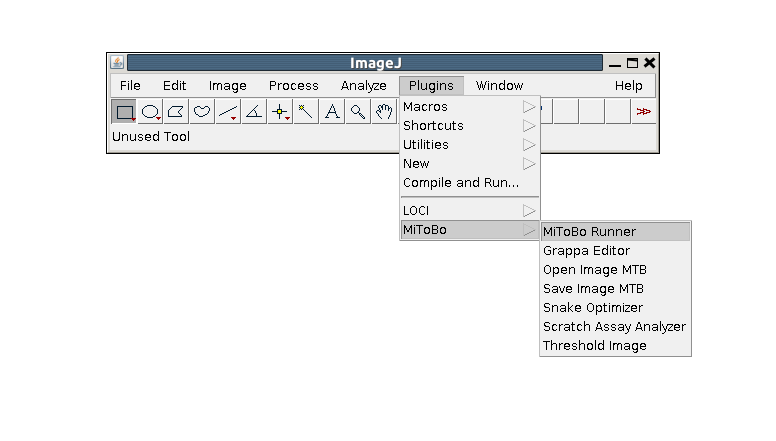
\includegraphics[width=0.85\textwidth,clip,trim= 0 0 0 30]{../images/ScreenshotImageJ_trans.png}
\vspace*{-1.7cm}
\caption{\label{fig:imageJ}Screenshot of ImageJ's plugin menu including \mitobo's submenu.}
\end{center}
\vspace*{-0.25cm}
\end{figure}
\end{center}

\vspace*{-0.75cm}
As mentioned above the key component for accessing \mitobo's functionality from within ImageJ is
its operator runner. Fig.~\ref{fig:oprunner} shows a screenshot of its main window after it has 
been invoked from ImageJ's plugin menu\footnote{\mitobo also offers a toolbar button and an associated start-up macro
to enable direct access to the operator runner, please refer to the installation instructions on the webpage for details on 
how to setup the button.}.

\begin{wrapfigure}[19]{r}{0.5\textwidth}
\vspace*{-1.6cm}
\begin{center}
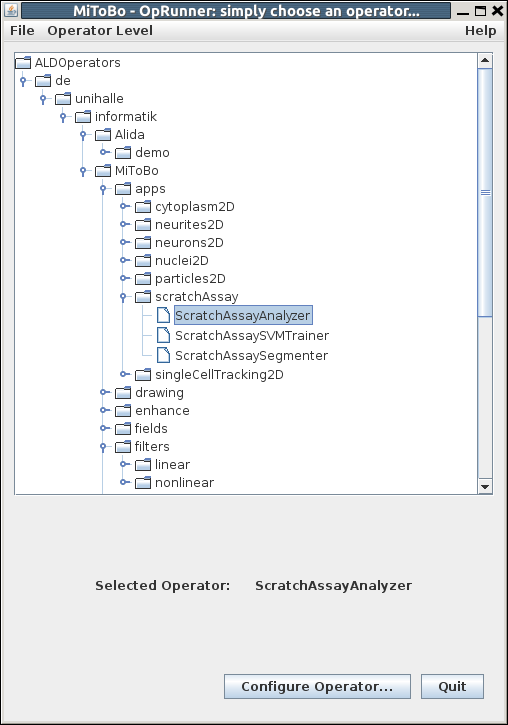
\includegraphics[width=0.475\textwidth]{../images/ScreenshotOpRunner.png}
\vspace*{-0.45cm}
\caption{\label{fig:oprunner}Screenshot of \mitobo's operator runner.}
\end{center}
\end{wrapfigure}
The operator runner basically displays a hierarchical menu of all available \alida and \mitobo
operators, organized according to their Java packages. From this menu you can select the 
operator of your choice, either by simply double-clicking on its name, or by selecting the entry
and clicking the 'Configure Operator \ldots' button at the bottom of the window. 
Subsequently \mitobo will launch a control window 
for the selected operator which allows you to configure and execute the operator you have chosen. 
Note that in \mitobo two different categories of operators are available. On the one hand there
are operators optimized for use by non-experts and often of general interest, while on the 
other hand it also subsumes a large collection of more sophisticated and often quite specific
operators. You can switch the operator selection menu between these categories via the 
item 'Operator Level' in the menubar on top of the window.
  
%\begin{wrapfigure}[15]{r}{0.65\textwidth}
%\vspace*{-0.5cm}
%\begin{center}
%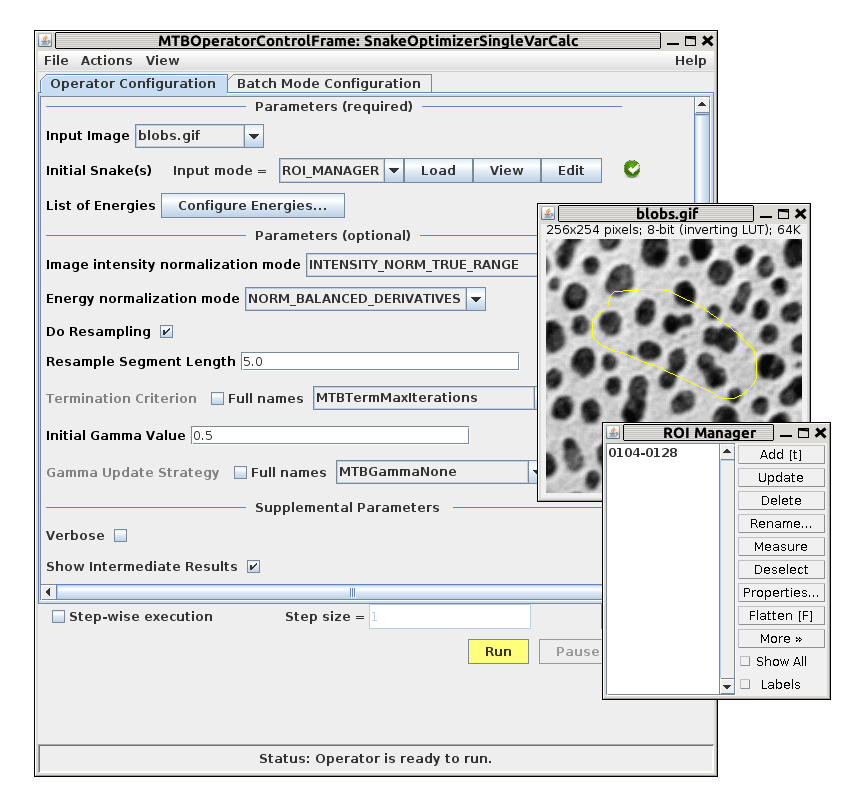
\includegraphics[width=0.6\textwidth]{../images/ScreenshotSnakeOp_trans.png}
%\caption{\label{fig:snakeop}Screenshot of the control window for the Snake Optimizer operator.}
%\end{center}
%\end{wrapfigure}
\begin{center}
\begin{figure}[t]
\begin{center}
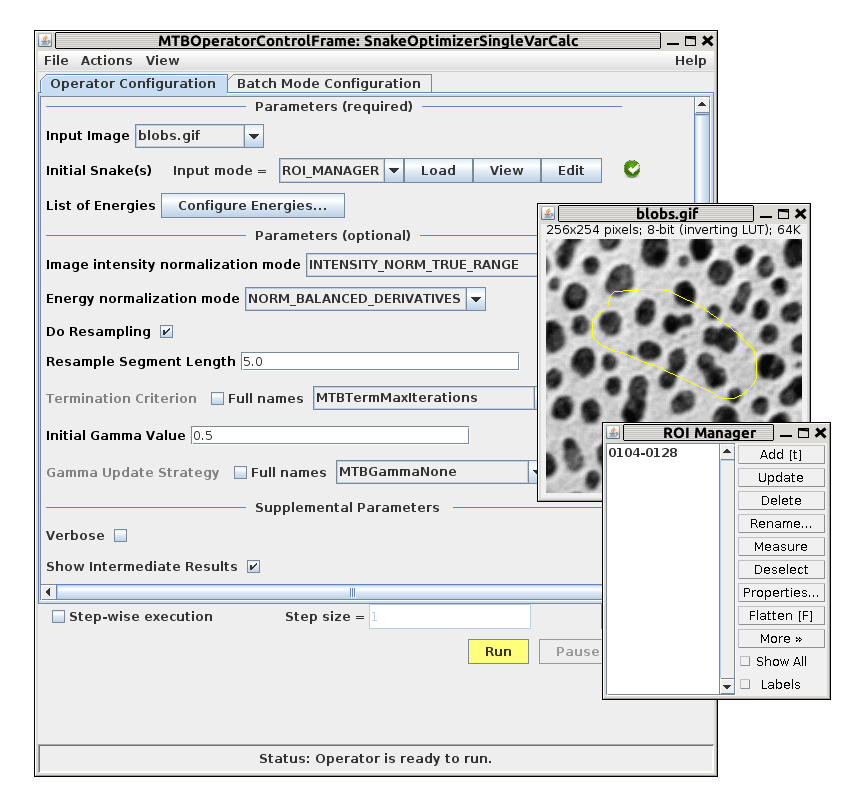
\includegraphics[width=0.85\textwidth]{../images/ScreenshotSnakeOp_trans.png}
\caption{\label{fig:snakeop}Screenshot of the control window for the 'Snake Optimizer' operator.}
\end{center}
\end{figure}
\end{center}

In Fig.~\ref{fig:snakeop} as an example the control window for the 'Snake Optimizer' operator is depicted.
It is automatically generated by the framework from the operator's source code and allows for 
operator configuration and execution. The window basically displays a panel with graphical
elements to configure all the parameters of the operator. It offers a menubar where you can 
find items for loading and saving the operator configuration, change viewing options, and also have
access to an online help for the specific operator. The help provides detailed information on the 
operator's parameters and how to configure the operator properly. The bottom section of the control
window contains control elements for executing the operator. In the simplest case there is just
a 'Run' button. More sophisticated operators, like the 'Snake Optimizer', allow for advanced user interaction.
For these operators the panel includes additional buttons, e.g., for pausing and resuming the operator. 
